%============================== Início Retomada ==========================

\textcite{harrod_essay_1939} apresenta um aparato teórico que permite analisar modelos em sua forma dinâmica sem precisar recorrer à defasagens entre as variáveis. Apresenta uma equação que engloba tanto o efeito multiplicador quanto o princípio acelerador cuja implicação é que o equilíbrio dinâmico não é estável. Diante desta problemática, surgiram os modelos de Cambridge, Kaleckianos e supermultiplicador sraffiano na tentativa para domar tal instabilidade (ver tabela \ref{crescimento}). Na seção \ref{SecHarrod}, foram apresentadas tais alternativas em que o modelo de Cambridge não se mostrou adequado dadas as incompatibilidades com o comportamento das firmas associada a essa teoria. Desse modo, restaram os modelos kaleckianos e o SSM. 

A seção seguinte abordou a controvérsia em torno do grau de utilização e sua convergência ao normal no longo prazo e as implicações para os paradoxos dos custos e da parcimônia. Além disso, foram realçadas algumas críticas aos modelos Kaleckianos relacionadas a convergência/endogeinização ao/do grau de utilização normal. Argumenta-se que um modelo que privilegia o PDE no longo prazo deve reportar o fato estilizado reportado acima uma vez que implica no equilíbrio (dinâmico) estável entre crescimento e capacidade produtiva. Neste ponto, cabe destacar a seguinte passagem de \textcite[p.~120, grifos nossos]{serrano_sraffian_1995}:

\begin{citacao}
Indeed, the true reason for the lack of balance between capacity and demand in the Oxford theory [Modelos kaleckianos] in the long run is actually much simpler. As we have seen above in this theory, in the long run the level of output adapts itself to the level of aggregate demand. The level of productive capacity, however, cannot adjust to this level of aggregate demand because current capacity has already been determined as the result of previous autonomous investment. Hence it is the idea that investment is \textbf{autonomous} and not \textbf{anything related to oligopoly} or competition that explain the long-run discrepancies between capacity and demand.
\end{citacao}
Nesses termos, os modelos kaleckianos tradicionais foram descartados. Como será argumentado a seguir, tal decisão decorre das implicações de se considerar o investimento enquanto variável autônoma no médio  e longo prazo.

Coube a seção \ref{Literatura} apresentar a resposta kaleckiana a crítica envolvendo o pricípio do ajuste do estoque de capital em que foram incluídos gastos autônomos não criadores de capacidade. Para encerrar essa discussão, é feita uma comparação entre as duas alternativas restantes, qual sejam, Kalekiana não-convencional e Sraffiana. Em linha com \textcite{fagundes_role_2017}, argumenta-se que no \textbf{longo prazo} os modelos kaleckianos não-convencionais respondem suficientemente bem à convergência do grau de utilização sem incorrer na instabilidade de Harrod. Diante disso, existem duas questões importantes em aberto: (i) dadas as hipóteses compartilhadas, qual a distinção fundamental entre ambos os modelos? (ii) dados os objetivos desta investigação, qual modelo a ser adotado? Resta a esta seção responder tais questões. Antes de prosseguir para a seleção do modelo a ser usado, serão destacadas algumas questões envolvendo o supermultiplicador sraffiano. 

%=================================================================================
%								Tabela: modelos de crescimento
%=================================================================================
\begin{table}[htb]
	\centering
	\caption{Fechamento das principais teorias de crescimento heterodoxas}
	\label{crescimento}
	\resizebox{\textwidth}{!}{%
		\begin{tabular}{|l|ccccl|}
			\hline 
			\textbf{Modelo} & \begin{tabular}[c]{@{}c@{}} \textbf{Regime de} \\\textbf{crescimento} \end{tabular} &  \begin{tabular}[c]{@{}c@{}} \textbf{Distribuição} \\\textbf{de renda} \end{tabular} & \begin{tabular}[c]{@{}c@{}}\textbf{Grau de utilização} \\ \textbf{da capacidade}\end{tabular} & \begin{tabular}[c]{@{}c@{}} \textbf{Capacidade}  \\ \textbf{produtiva} \end{tabular} & \textbf{Fechamento} \\ \hline
			\textbf{Cambridge} & Ausente  & Endógena & \begin{tabular}[c]{@{}c@{}} Exógena \\ \end{tabular} & Exógena & Distribuição de renda\\
			\textbf{Kaleckiano} & Wage/Profit-led &  \begin{tabular}[c]{@{}c@{}} Exógena \\ (\textit{Mark-up}) \end{tabular} & Endógena   & Exógena & Grau de utilização \\ 
			\begin{tabular}[l]{@{}l@{}}\textbf{Supermultiplicador} \\\textbf{Sraffiano} \end{tabular} & Ausente & \begin{tabular}[c]{@{}c@{}} Exógena \\ (Teoria Monetária\\da distribuição)  \end{tabular} & Tende ao normal & Endógena & \begin{tabular}[c]{@{}c@{}} Propensão média \\ a poupar \end{tabular} \\ \hline
		\end{tabular}%
	}
\caption*{\textbf{Fonte:} Elaboração própria}
\end{table}


%============================== Fim Retomada ==========================

%CRÍTICAS DE NIKIFOROS
Em sua crítica, \textcite{nikiforos_comments_2018} destaca os seguinte pontos: 
(i) os gastos autônomos podem ser incorporados nos modelos kaleckianos e, portanto, os resultados para o curto e médio prazo não são inéditos; 
(ii) é um modelo de longo prazo e deve ser avaliado enquanto tal; 
(iii) no longo prazo, é o grau de utilização normal que se endogeiniza; 
(iv) investimento apesar de não depender da poupança, não desempenha um papel relevante; 
(v) no longo prazo, $Z$ deixa de ser autônomo\footnote{Os pontos (i) e (iii) já foram abordados indiretamente ao longo da exposição enquanto os demais devem ser analisados mais detidamente.}.  No que diz respeito ao ponto (i), toda a discussão feita nesta seção indica que os gastos autônomos podem sem ser incluidos nos modelos kaleckianos, enquanto no longo prazo deve ser válido o princípio do ajuste do estoque de capital para não incorrer na instabilidade Harrodianda. 

No que diz respeito à convergência ao grau de utilização ao nível normal, \citeauthor*{nikiforos_comments_2018} afirma:

\begin{citacao}

[T]he acceptance that in the long run the economy converges to a supply-determined rate of utilization means that either the role of demand vanishes and the model becomes ``classical in the long run'' (Duménil and Lévy 1999), or that demand remains independent but distribution becomes endogenous to allow for the convergence. \cite[p.~9]{nikiforos_comments_2018}
\end{citacao}
Tal raciocínio é infundado por duas razões: (i) convergência ao grau de utilização normal não implica que a demanda é irrelevante. De acordo com o supermultiplicador sraffiano, é a capacidade produtiva que se ajusta à demanda e não o inverso; (ii) se o grau de utilização converge ao normal, a distribuição de renda não é endogeneizada e isso é verificado pela endogeinização da propensão média a poupar decorrente de $Z>0$.

No que diz respeito aos gastos autônomos, o item (v) é o mais problemático e, portanto, esclarecê-lo permite uma melhor compreensão dos anteriores. Ao longo de seu artigo, \textcite[p.~4]{nikiforos_comments_2018} mescla a noção de autônomia com a de exogeneidade\footnote{Uma forma de verificar ambiguidade na definição de Nikiforos é que nos modelos kaleckianos analisados nesta seção tornam o investimento induzido no longo prazo por meio da endogeinização do parâmetro $\gamma$, antes autônomo. }: ``\textit{Autonomous means that is not affected by other economic variables within the system}''. Em linhas gerais, autonomia pode ser associada a independência relativa das demais variáveis econômicas enquanto exogeneidade é uma independência absoluta. Como destacado anteriormente, um gasto é considerado autônomo se independer das decisões de produção (renda) enquanto \textcite{serrano_sraffian_1995} acrescenta a não criação de capacidade produtiva a essa categorização. 

A incompreensão reportada anteriormente pode ser verificada no item (iv) em que afirma que uma das implicações da resolução da instabilidade de Harrod \textit{à la} supermultiplicador é a quase-endogeinização do investimento. No entanto, seguindo o princípio de ajuste do estoque de capital, o investimento se torna \textbf{induzido} (inverso de autônomo) e não endógeno (inverso de \textbf{exógeno}). Partindo da noção de autonomia apresentada anteriormente, \citeauthor*{nikiforos_comments_2018} afirma:
\begin{citacao}

[N]one of the arguments of the investment function play any role whatsoever in the long run. This is strangely
reminiscent of supply-side models or the FKP [Modelo de Cambrigde] where the accumulation rate converges to the
exogenous natural growth rate in the long run. \cite[p.~11--12, comentario adicionado]{nikiforos_comments_2018}
\end{citacao}
O modelo do supermultiplicador, no entanto, não afirma que o investimento deixa de ser relevante. \textcite{dejuan_hidden_2017}, por exemplo, destaca que as economias que apresentam uma maior taxa de crescimento são aquelas com uma maior taxa de investimento e não aquelas com grau de utilização persistentemente mais elevado. A maior taxa de investimento, por sua vez, é um resultado esperado do supermultiplicador uma vez que a participação dos gastos autônomos na renda diminui diante de uma taxa de crescimento destes gastos ampliada.

Resta, portanto, a questão referente a temporalidade do supermultiplicador. O argumento de \citeauthor*{nikiforos_comments_2018} é que tal modelo é adequado somente para o longo prazo. No entanto, uma vez que $Z$ deixa de ser autônomo (como visto, exógeno), passa a ter a capacidade explicativa comprometida, ou nas palavras do autor, ``\textit{a cart without its horse}''. Dois pontos desta afirmação devem ser reformulados diante da discussão anterior a despeito do supermultiplicador sraffiano: (i) no longo prazo, $Z$ permanece autônomo e, portanto, continua sendo um modelo válido; (ii) por mais que tenha sido desenvolvido para tratar de questões de longo prazo não impede de utilizá-lo para analisar o ciclo econômico. 

Feitas estas ressalvas, é possível avançar para as questões levantadas anteriormente.  O primeiro ponto pode ser respondido de forma mais direta: a principal diferença é a autonomia do investimento no curto e médio prazo.  Resumidamente, se o investimento produtivo for induzido, a convergência ao grau de utilização é uma derivação do princípio do ajuste do estoque de capital e, dados certos limites, a capacidade produtiva se ajusta à demanda efetiva. Por outro lado, se o investimento possuir um componente autônomo, como nos modelos kaleckianos convencionais, a demanda efetiva se ajusta à capacidade produtiva que está definida aprioristicamente. Como a seção \ref{Literatura} mostrou, isso deixa de ser o caso nos modelos kaleckianos com investimento induzido no longo prazo.

Para responder a segunda questão, resta esclarecer um possível ponto de estranhamento. O principal objetivo desta pesquisa é investigar os determinantes do ciclo econômico norte americano e desenvolver um modelo que replique alguns dos fatos estilizados. Sendo este o caso, a ênfase na discussão de modelos de longo prazo parece ser desconexa. No entanto, a escolha deste caminho argumentativo decorre da convergência ao grau de utilização normal como um critério de seleção. Desse modo, optar por modelos que se mostram adequados para o curto e médio prazo, mas não para o longo se mostra questionável uma vez que a validade dos resultados está restrita a uma certa temporalidade. Como mencionado na introdução, os modelos elegíveis são aqueles reportam alguns fatos estilizados (\textit{e.g.} relação positiva entre taxa de investimento e crescimento)  no curto, médio e longo prazo.

Como visto, ambas famílias de modelos preservam tal característica no curto e longo prazo. Resta verificar se o mesmo vale para \textbf{médio prazo}. Dito isso, dentre os modelos kaleckianos com gasto autônomos e com principio de ajuste do estoque de capital e supermultiplicador sraffiano, resta selecionar aquele reproduza o fato estilizado da relação positiva entre taxa de investimento e taxa de crescimento \cites[p.~172]{cesaratto_neo-kaleckian_2015}[p.~8--9]{fiebiger_trend_2017}\footnote{Esta parte da exposição é inspirada na contribuição de \textcite{fagundes_role_2017} no que diz respeito ao médio prazo.}. Dito isso, seja $h$ a propensão marginal a investir, $i$ a taxa de investimento e $\gamma_A$ a parcela autônoma do investimento de modo que a função de acumulação kaleckiana e supermultiplicador (adiante, SSM) se tornam:

$$
\frac{I}{K}  = \gamma + \gamma_uu - \gamma_uu_N
$$


\begin{equation}
    \tag{kaleckiana}
I = (\gamma_A + \gamma_uu)K \Rightarrow I = (\gamma_A + \overbrace{h}^{\gamma_u\cdot v}\cdot u)K
\end{equation}

\begin{equation}
    \tag{SSM}
    i = \frac{I}{Y} \Leftrightarrow I = h\cdot Y
\end{equation}
Como destacado na seção \ref{SecHarrod}, na ausência de gastos autônomos, a propensão marginal e média a poupar são iguais e, portanto, no modelo kaleckiano convencional, a taxa de investimento é determinada pela taxa de poupança definida exogenamente. Incluindo tais gastos no modelo, obtém-se:

$$
i = \frac{i_{Trad}\gamma_A + hz}{\gamma_A + z}
$$
em que $i_{Trad}$ denota, tal como em \textcite{fagundes_dinamica_2017}, a taxa de investimento no modelo kaleckiano canônico e, assim, outra diferença entre os modelos é explicitada. Nos modelos kaleckianos com modificações, a ausência dos gastos autônomos implica na volta ao modelo kaleckiano convencional enquanto no supermultiplicador, com $Z = 0$ retorna-se ao \textcite{harrod_essay_1939}. Mais uma vez, a introdução de $Z$ não é capaz, por si só, de eliminar a instabilidade dos modelos kaleckianos mas sim pela modificação da função investimento no longo prazo. 

Prosseguindo com a exposição e analisando o equilíbrio de \textit{steady growth} com $Z > 0$, verifica-se que no médio prazo dos modelos kaleckianos não-convencionais ($g\to g_Z$) a taxa de investimento ($i_{MR}$) é dada por:
\begin{equation}
    \label{investoFagundes}
i_{MR} = \frac{hg_Z}{g_Z - \gamma_A}
\end{equation}
Diante deste resultado, \textcite{fagundes_role_2017} argumentam que a inclusão de $Z$ no modelo não garante a convergência do grau de utilização ao normal. Para que tal tendência ocorra, por sua vez, é necessário que a participação da parcela autônoma do investimento convirja a zero ($\gamma_A \to 0$). 
Adicionalmente, \textcite{fagundes_role_2017} reportam uma relação negativa entre taxa de crescimento e taxa de investimento. Supondo, por simplificação, que as variações são infinitesimais, isto pode ser explicitado em termos da equação \ref{investoFagundes} por derivadas parciais:
$$
\frac{\partial i_{MR}}{\partial g_Z} = - \frac{\gamma_A h}{[g_Z - \gamma_A]^2} < 0 \Leftrightarrow \gamma_A > 0
$$
Além disso, os autores pontuam um problema de ``dupla indentidade'' no modelo decorrente das diferentes condições de equilíbrio, um em $Z = 0$ e no outro $Z>0$, cujos padrões de crescimento são mutualmente excludentes. No primeiro, obtém-se um regime liderado pelo investimento mas incapaz de gerar a tendência do grau de utilização ao normal e de destacar a importância dos gastos autônomos ($Z\to 0$). No outro, ocorre o inverso, um regime liderado pelos gastos autônomos ($\gamma_A \to 0$) mas que evidencia uma relação negativa entre crescimento e taxa de investimento. Ambos os casos, contraria-se os fatos estilizados. Portanto, a aceitação a conclusão de \textcite[p.~13]{fagundes_role_2017} é imediata:

\begin{citacao}

[I]f we think of such a model as an intermediate step towards the long-run model, then we
believe that there is no problem in using it. The problem occurs when we think of the medium-run
model as a contribution to the understanding of economic reality in itself, independent from the long-
run model.
\end{citacao}

Resta checar se a alternativa pelo SSM incorre nos mesmos problemas. Para isso, basta verificar os resultados para o caso em que o investimento é completamente induzido. Como a alternativa kaleckiana com gastos autônomos pode ser considerada como híbrida entre o modelo kaleckiano convencional e o SSM, substituindo $\gamma_A = 0$ na equação \ref{investoFagundes}, obtém-se:
$$
i_{MR} = \frac{I}{Y} =  h
$$
Seguindo a proposta do supermultiplicador em que o investimento é completamente induzido:
$$
g = \frac{h\cdot u}{v} \Rightarrow h = i_{MR} = \frac{g\cdot v}{u}
$$

$$
\frac{\partial i_{MR}}{\partial g} = \frac{v}{u} > 0
$$
Portanto, a relação negativa entre crescimento e taxa de investimento deixa de existir e isso não é feito às custas da não convergência do grau de utilização ou da relevância dos gastos autônomos no longo prazo. Neste ponto, o trecho a seguir é esclarecedor:

\begin{citacao}
 What the supermultiplier adds to the neo-Kaleckian framework is a plausible mechanism for explaining phases
of the business cycle when the output share of capacity investment is rising amidst robust rates of output growth. \cite[p.~9]{fiebiger_trend_2017}
\end{citacao}
Até então, pode-se dizer que a teoria do crescimento liderado pela demanda enfrentava um dilema. Não conseguia conciliar estabilidade, distribuição funcional da renda exógena e grau de utilização da capacidade produtiva igual ao normal/planejado, aparentando uma trindade impossível do crescimento, conforme pode ser visto no diagrama \ref{diagrama}\footnote{Este diagrama é inspirado no ``trilema'' do crescimento apresentado por \textcite{cesaratto_neo-kaleckian_2015}.}.


\begin{figure}[htb]
    \caption{Trindidade ``impossível''}
    \label{diagrama}
    \begin{center}
    \resizebox{0.45\textwidth}{!}{%
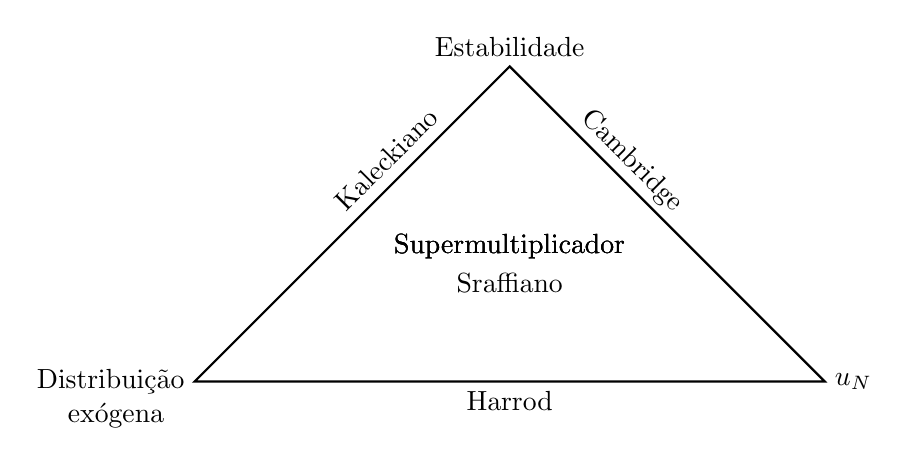
\begin{tikzpicture}[thick]
    \path[draw] (-4,0)  coordinate [label= left:Distribuição] (A)

            -- ( 0,4)  coordinate [label=above:Estabilidade] (C)
            -- ( 4,0)  coordinate [label=right:$u_N$] (B)
            -- cycle;
    \foreach \point in {A,B,C}
    \draw
        -- (0,2) node[anchor=north]{Supermultiplicador};
    \draw
        -- (-5,-0.15) node[anchor=north]{exógena};
    \draw
        -- (0,1.5) node[anchor=north]{Sraffiano};
    \draw
        -- (-1.75,3) node[anchor=north, rotate=45]{Kaleckiano};
    \draw
        -- (1.75,3) node[anchor=north, rotate=-45]{Cambridge};
    \draw
        -- (0,0) node[anchor=north]{Harrod};
\end{tikzpicture}
}
\end{center}
\caption*{\textbf{Fonte:} Elaboração própria}
\end{figure}
\noindent Essa trindade impossível se mostrou falsa com o desenvolvimento do supermultiplicador sraffiano, proposto por \textcite{serrano_long_1995} e \textcite{bortis_institutions_1996}. Portanto, diante da discussão anterior, conclui-se que o modelo do SSM não é incompatível para analisar o médio prazo ou restrito ao longo prazo como afirma \textcite{nikiforos_comments_2018}. Com isso, encerra-se este capítulo elegendo o supermultiplicador sraffiano como o mais adequado por replicar os fatos estilizados mencionados anteriormente e por validar o PDE no curto, médio e longo prazo. Seguindo a sugestão de \textcite[p.~280]{freitas_growth_2015}, esta investigação avança no sentido de contribuir para a compreensção de outros componentes da demanda agregada não criadores de capacidade. Destaca-se ainda que a instabilidade da economia não decorre da junção do acelerador com o multiplicador\footnote{Como mostram \textcite{serrano_trouble_2017}, dadas certas condições, o SSM é dinamicamente \textit{estável}.}, mas sim da própria instabilidade da demanda agregada \cite{dejuan_hidden_2017}.  Dito isso,  o capítulo seguinte irá esboçar alguns esforços para evidenciar a importância do investimento residencial para a dinâmica do ciclo econômico norte americano e, assim, preencher uma das lacunas dos modelos de crescimento com gastos autônomos.






